%\chapter{det-comp}


%%%%%%%%%%%%%%%%%%%%%%%%%%%%%%%%%%%%%%%%%%%%%%
%\section{Anode Plane Assemblies}

%%%%%%%%%%%%%%%%%%%%%%%%%%%%%%%%%%%%%%%%%%%%%%
%\section{Cathode Plane Assemblies}

%%%%%%%%%%%%%%%%%%%%%%%%%%%%%%%%%%%%%%%%%%%%%%
%\section{Field Cage (FC)}
%\label{detcompsec-fc}


%%%%%%%%%%%%
\subsubsection{FC to beam plug}
\label{subsec:fc-beamplug}

%The beam plug is installed between the field cage and primary membrane where the charged particle beam enters the cryostat. Its main function is to displace about 45 cm of passive LAr layer in that region to allow the particle beam to enter the active TPC region with minimal upstream material interactions. 

%To minimize the material interactions of the particle beam in the cryostat upstream of the TPC, a volume of LAr along the beam path (between the cryostat membrane and the FC) is displaced, and replaced by a less dense volume of dry nitrogen gas. The gas is contained within the \textit{beam plug}, a cylindrical glass-fiber composite pressure vessel, about 50\,cm in length and 22\,cm in diameter.


The LAr-displacement beam plug, a cylindrical glass-fiber composite pressure vessel, about 50\,cm in length and 22\,cm in diameter, is filled with nitrogen gas via a stainless steel line that extends to the top of the cryostat. It is illustrated in Figure~\ref{fig:beamplug}.
A pressure relief valve (or burst disk) is installed on the nitrogen fill line on the top of the cryostat (externally) to ensure the pressure inside the beam plug does not exceed the safety level of about 22\,psi. The nitrogen system schematic is shown in Figure~\ref{fig:beamplugN2}. 
%A component-level view of the beam plug is shown in Figure~\ref{fig:beamplug_components}.  
The beam plug is secured to the FC support structure as illustrated in Figure~\ref{fig:beamplug-fc}. The front portion of the beam plug extends  5\,cm into the active region of the TPC  through an opening in the FC. The FC support is designed with sufficient strength and stiffness to support the weight of the beam plug before filling, while it is suspended in air.  When the cryostat is filled with LAr, the beam plug is roughly neutrally buoyant.  The total internal volume of the beam plug is about 16 liters. 

%As illustrated in Figure~\ref{fig:beamplug}, it is a cylidrical glass-fiber composite pressure vessel about 50cm in length and  22cm in diameter. It is filled with dry nitrogen gas via a stainless steel line that extends to the top of the cryostat. The pressure inside the beam plug is maintained externally up to 25 psi from room to LAr temperatures. A pressure relief valve (or burst disk) is installed on the nitrogen fill line on the top of the cryostat (externally) to ensure the pressure inside the beam plug does not exceed the safety level. The component-level view of the beam plug is shown in Figure~\ref{fig:beamplug_components}.  The beam plug is secured to the field cage support structure as described in Section~\ref{subsec:fc-beamplug}. The front portion of the beam plug extends 5~cm beyond the profiles to inside the active region of the TPC through an opening on the field cage. The field cage support is designed with sufficient strength and stiffness to support the weight of the beam plug while it is suspended in air.  When the cryostat is filled with LAr, the beam plug is roughly neutrally buoyant.  The total internal volume of the beam plug is about 16 liters. 

The requirements on the acceptable leak rate is between $7.8\times 10^{-5}$ scc/s and $15.6\times 10^{-5}$ scc/s. This is very conservative and is roughly equivalent to leaking  15\% of the nitrogen in the beam plug over the course of a year.
  In the worst-case scenario in which all the nitrogen in the beam plug leaks into the LAr cryostat, the increase in concentration is about 0.1\,ppm, which is still a factor of 10 below the maximum acceptable level, as specified by light detection requirements.
%  \fixme{need some reference with details for this requirement}
  At nominal operation, the voltage difference across the beam plug (between the first and the last grading ring) is 165\,kV. 

    To minimize risk of electrical discharges, the beam plug is divided into sections, each of which is bonded to stainless steel conductive grading rings. The seven grading rings are connected in series with two parallel paths of resistor chains. The ring closest to the FC is electrically connected to one of the FC profiles. 
  The ring nearest the cryostat wall is grounded to the cryostat inner membrane via a short grounding cable. 
%  A likely candidate is the high-voltage Super Mox 15-G$\Omega$ resistor by OHMITE. 
The maximum total power dissipated by the resistor chain is about 0.6\,W.


\begin{cdrfigure}[Beam plug]{beamplug}{The beam plug is a  composite pressure vessel filled with dry nitrogen gas. The vessel is about 50\,cm in length and about 22\,cm in diameter. The pressure vessel is divided into sections with each section bonded to a stainless steel grading ring. The grading rings are connected by three parallel paths of resistor chain.}
  \includegraphics[width=0.75\textwidth]{BeamPlug.pdf}
\end{cdrfigure}

%\begin{cdrfigure}[Beam plug component-level view]{beamplug_components}{Component-level view of the beam plug showing alternating electrode and composite ring structure.}
%  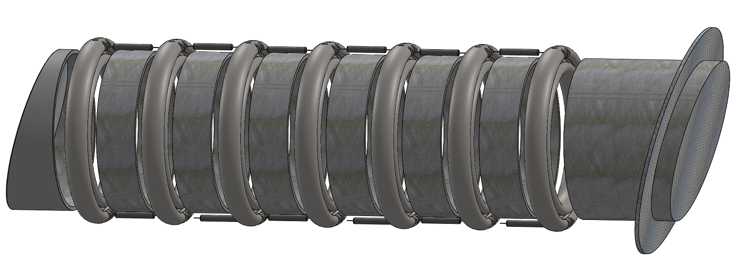
\includegraphics[width=0.7\textwidth]{beamplug_components.png}
%\end{cdrfigure}

\begin{cdrfigure}[Beam plug nitrogen system]{beamplugN2}{Beam plug nitrogen gas system schematics. The Local Control Panel is mounted on top of the cryostat near the DN160 flange feedthrough. The nitrogen line enters the cryostat via the 6-way flange which also has a burst disk for emergency pressure relief and temperature/pressure sensors.  }
  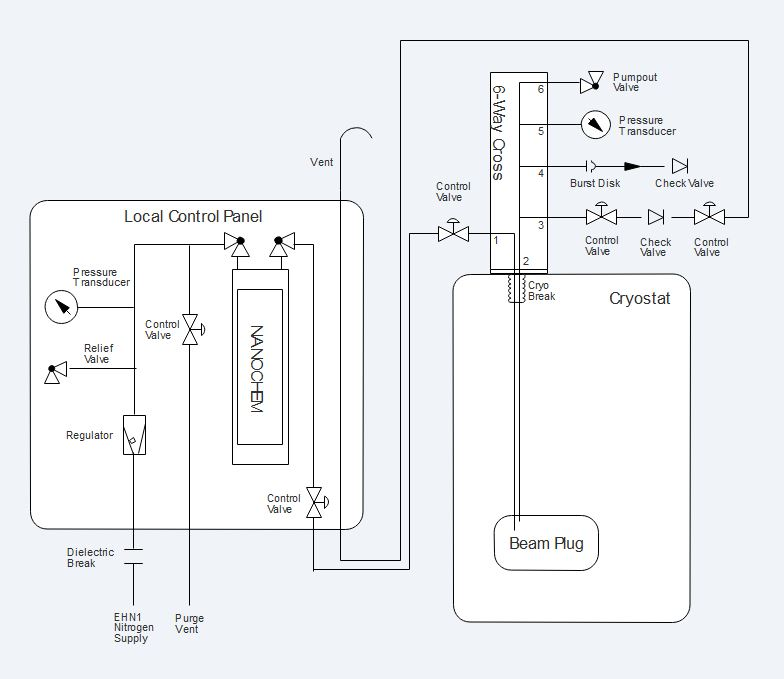
\includegraphics[width=0.75\textwidth]{beamplug_N2System.jpg}
\end{cdrfigure}

The metal electrode rings are spaced at regular intervals and interspersed with composite tube sections. The shape of the rings has been designed to minimize high electric field corners. The results of the field calculations are shown in Figures~\ref{fig:beamplug_ring1} and~\ref{fig:beamplug_ring2}. The average field in the vicinity of the beam plug is about 4.4\,kV/cm. The maximum field of 15.7\,kV/cm is on the electrode ring surface. In all regions the field is well below the 30-kV/cm limit.
%\fixme{citation to doc describing limit would be good}

\begin{cdrfigure}[Beam plug electrodes]{beamplug_ring1}{Electric field calculation of the electrode ring design. The average field in the beam plug region is about 4.4 kV/cm. The maximum field of 15.7\,kV/cm is on the electrode ring surface. }
  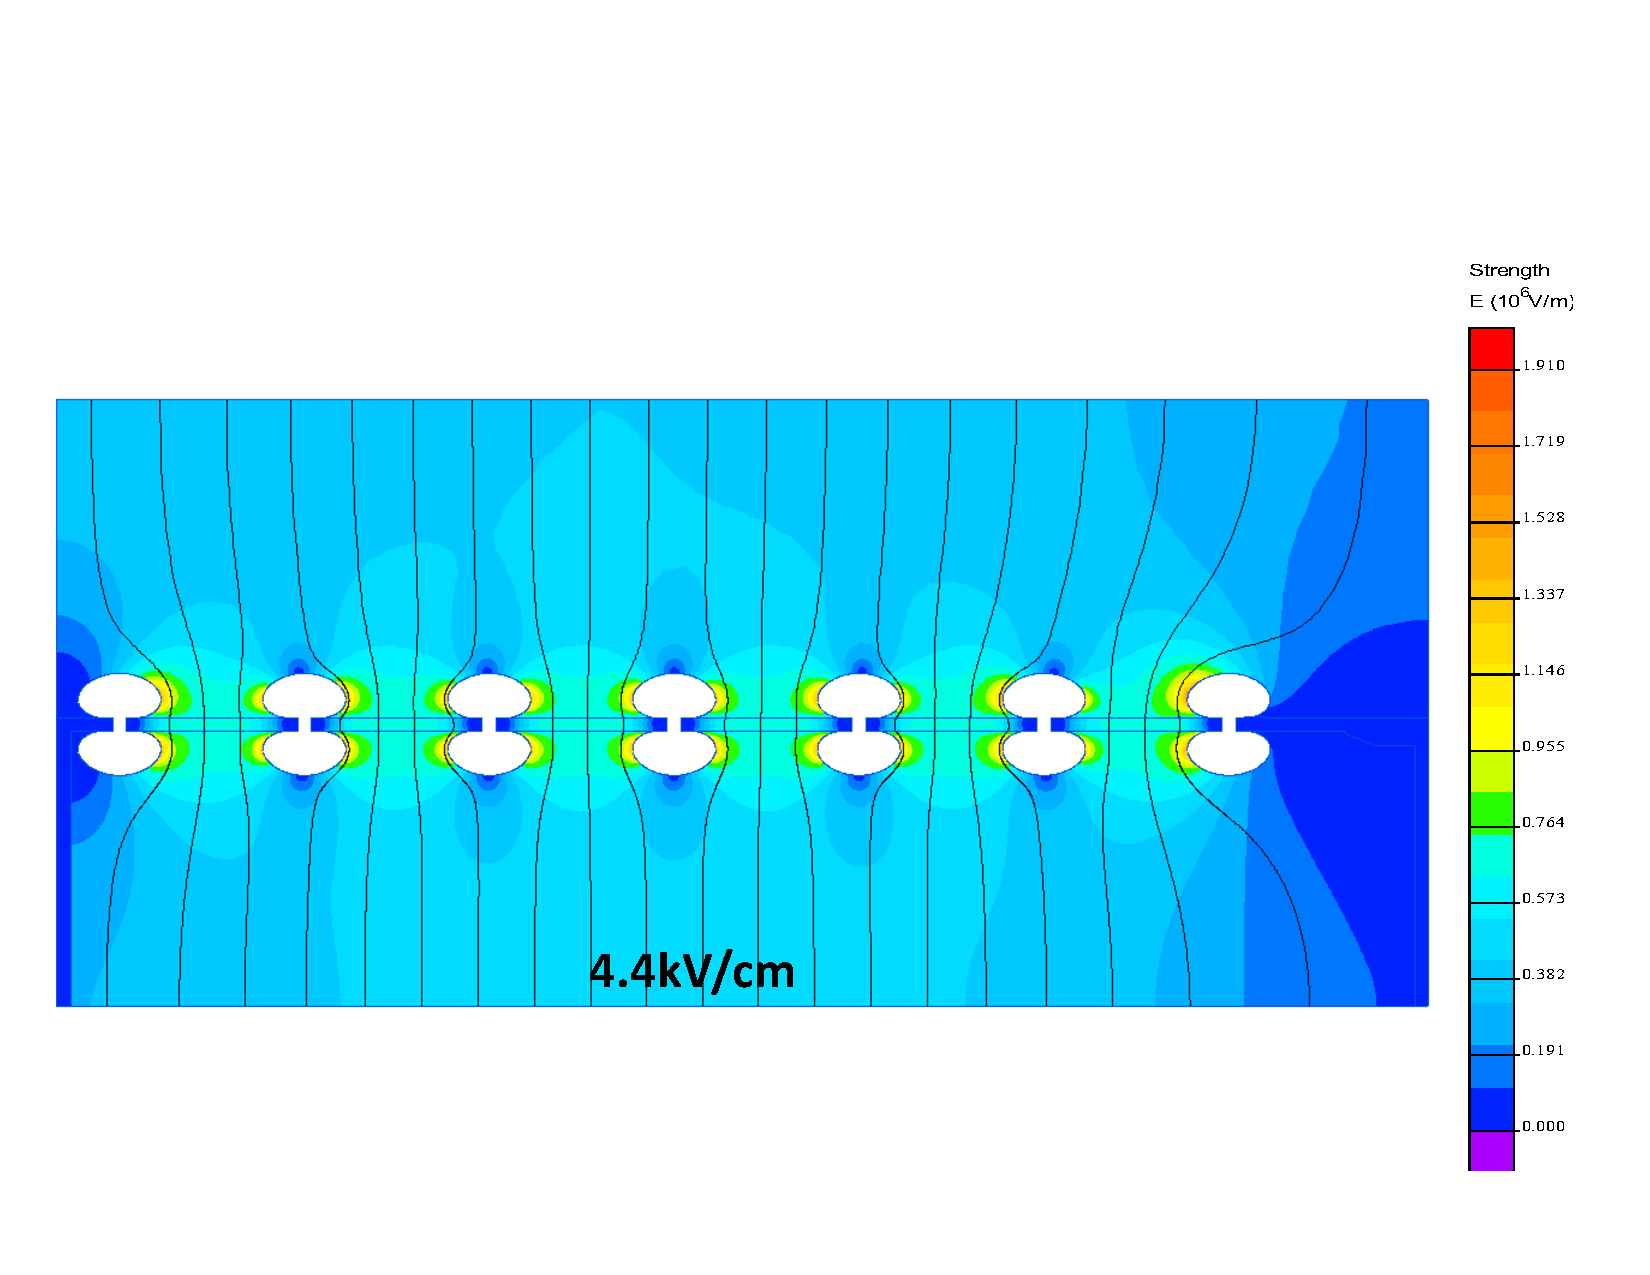
\includegraphics[width=0.85\textwidth]{beamplug_ring1.pdf}
\end{cdrfigure}

\begin{cdrfigure}[Beam plug electrode]{beamplug_ring2}{Electric field calculation near the vicinity of the electrode. The shape of the ring minimizes the high field region near the joints between the electrode, LAr, and composite shell. The field is well below the 30-kV/cm limit in all regions.}
  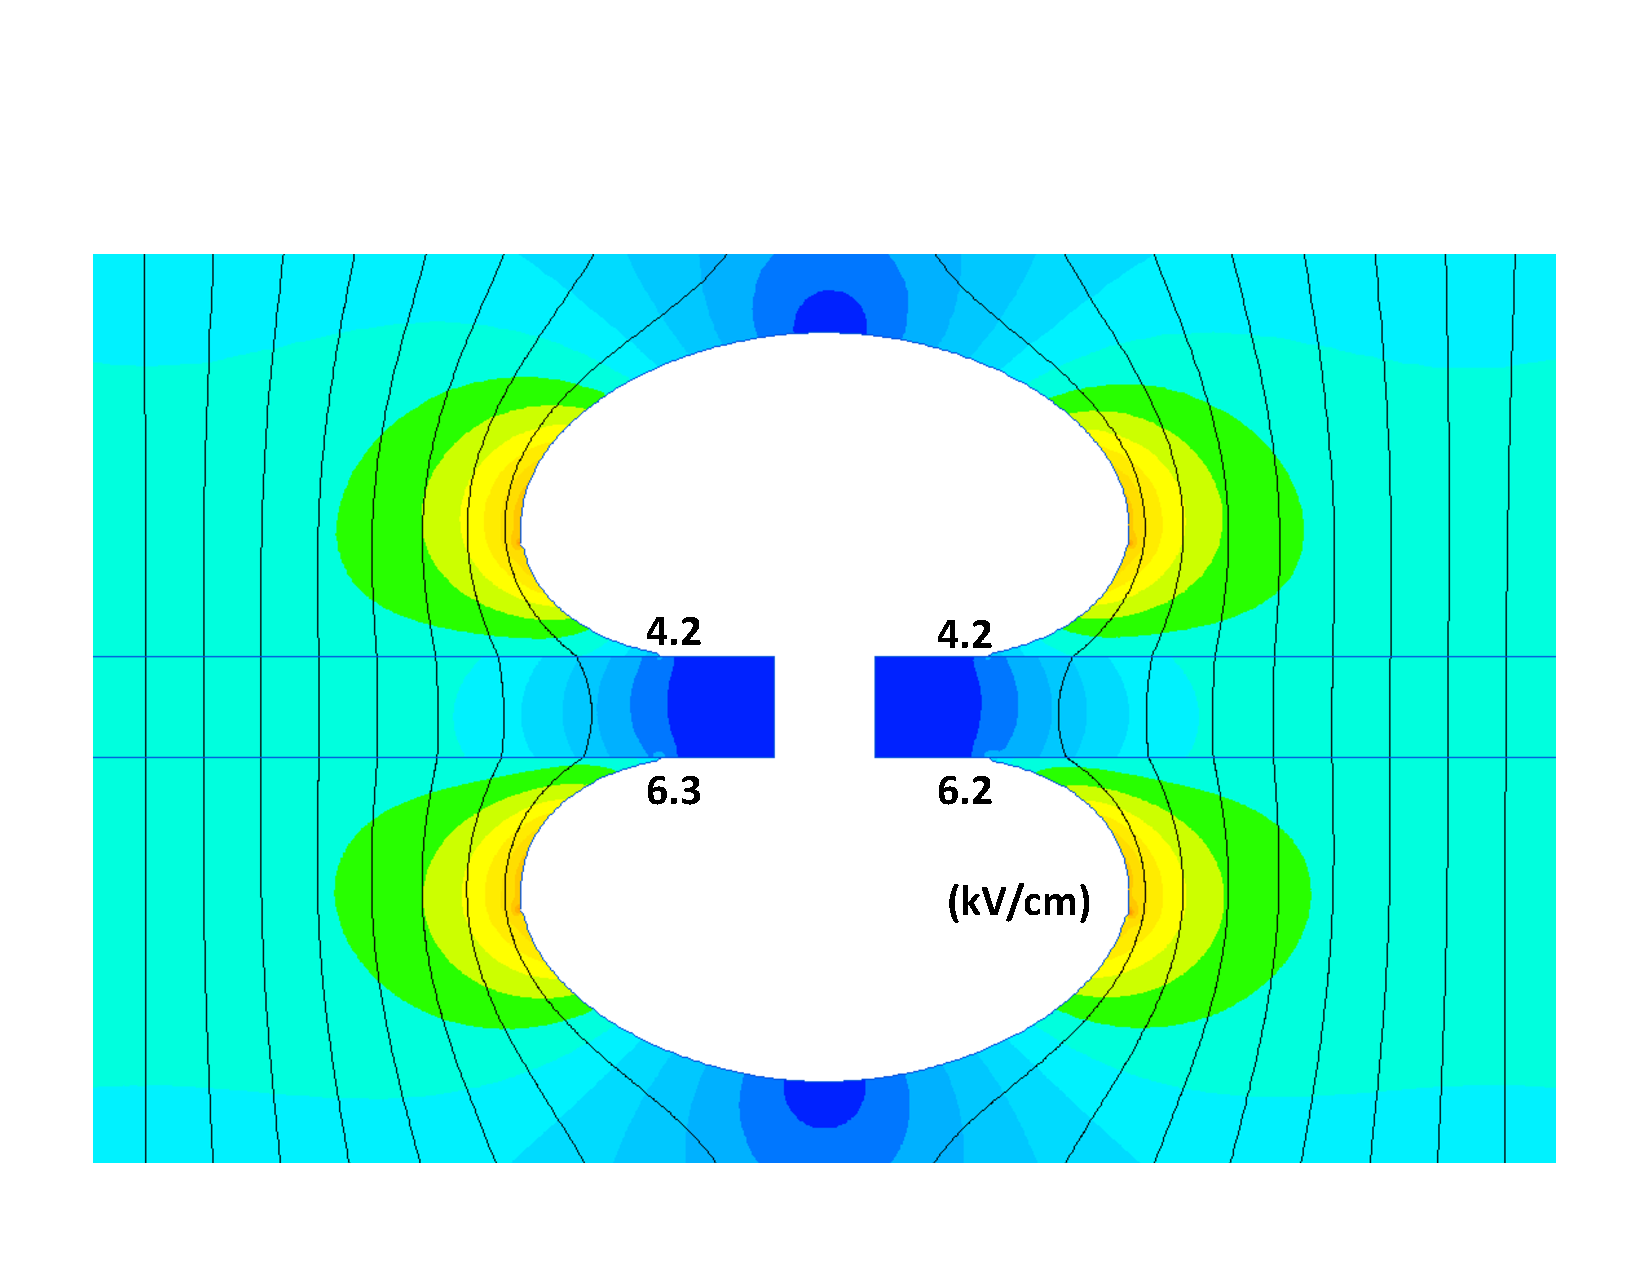
\includegraphics[width=0.5\textwidth]{beamplug_ring2.pdf}
\end{cdrfigure}

The beam plug is mounted onto one of the field cage support structures as shown in Figures~\ref{fig:beamplug-fc} and~\ref{fig:beamplug-fc2}. 
\begin{cdrfigure}[Beam plug to CPA connection]{beamplug-fc}{Beam plug to field cage interface.}
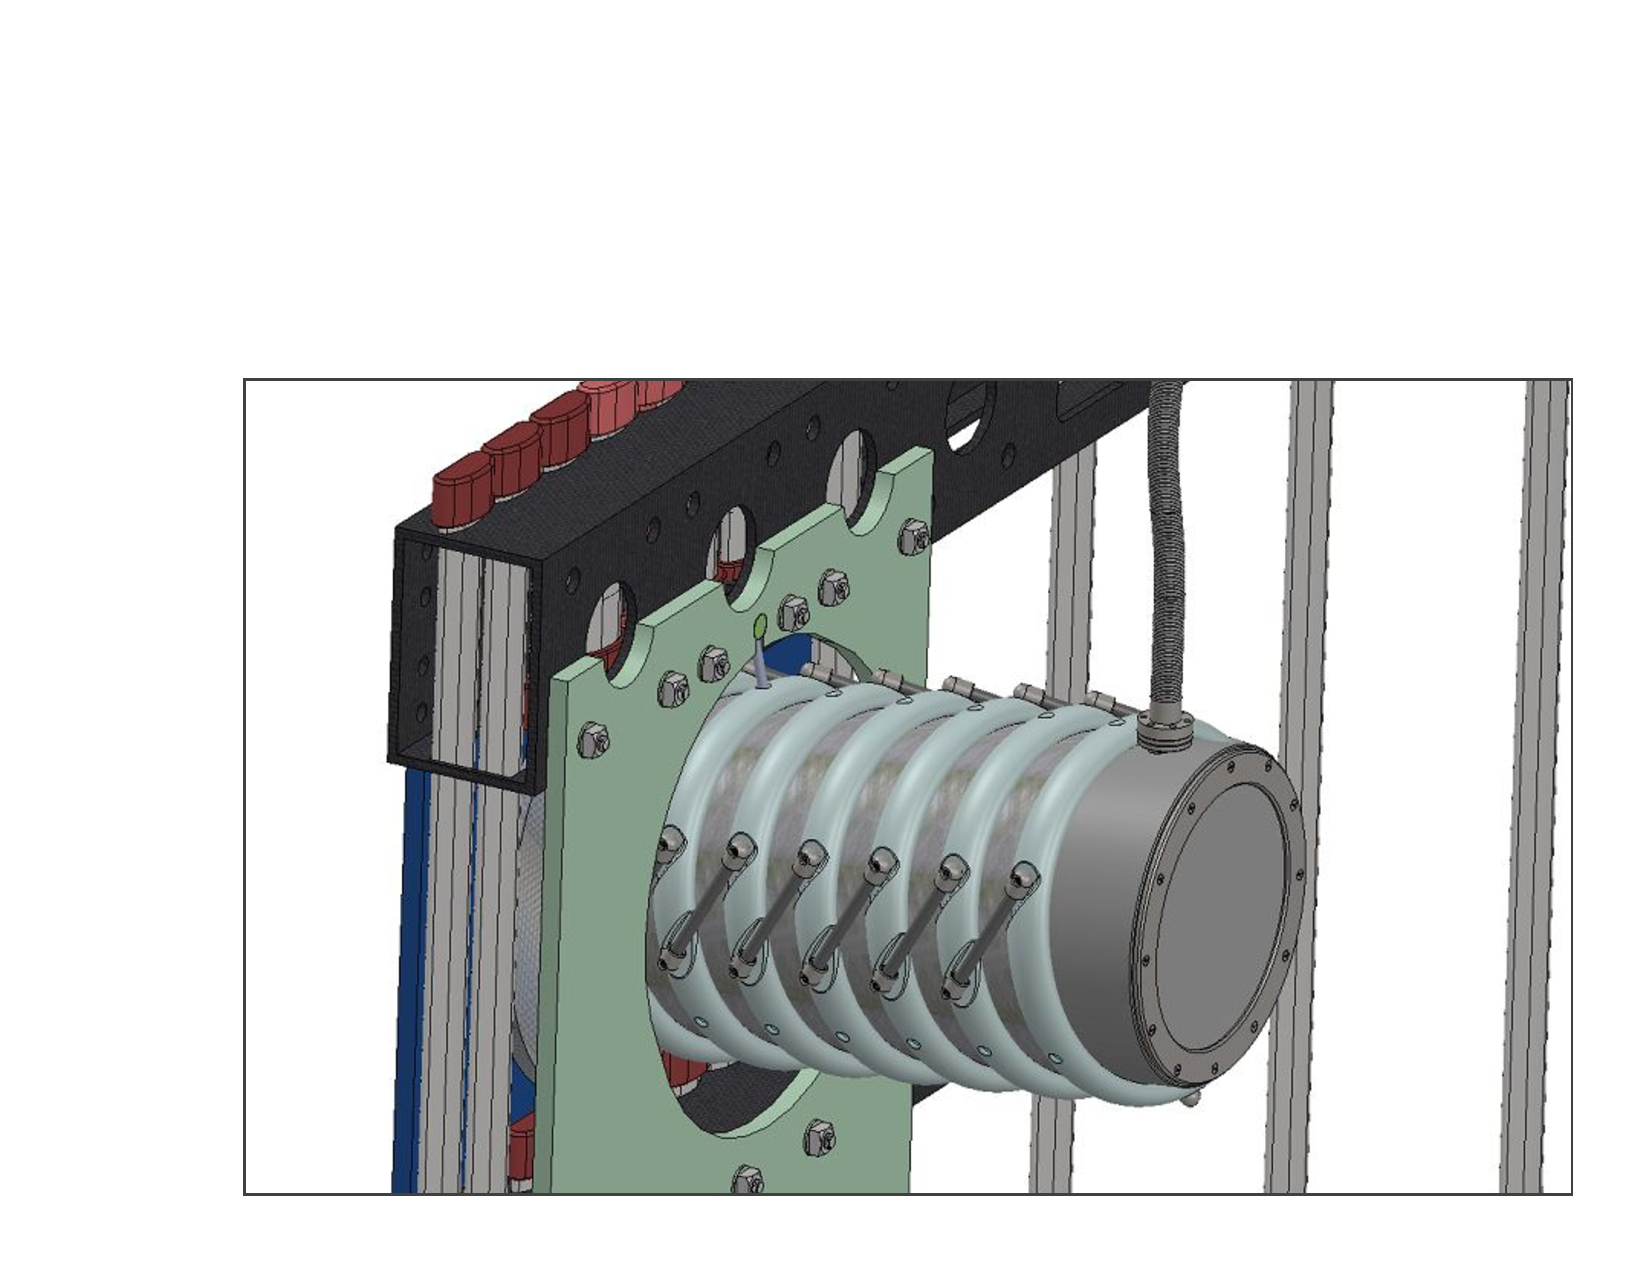
\includegraphics[width=0.75\linewidth]{beamplug_FC.pdf}
\end{cdrfigure}
%\begin{cdrfigure}[Beam plug to CPA connection]{beamplug-fc2}{Cutaway sideview of the beam plug to field cage interface.}
%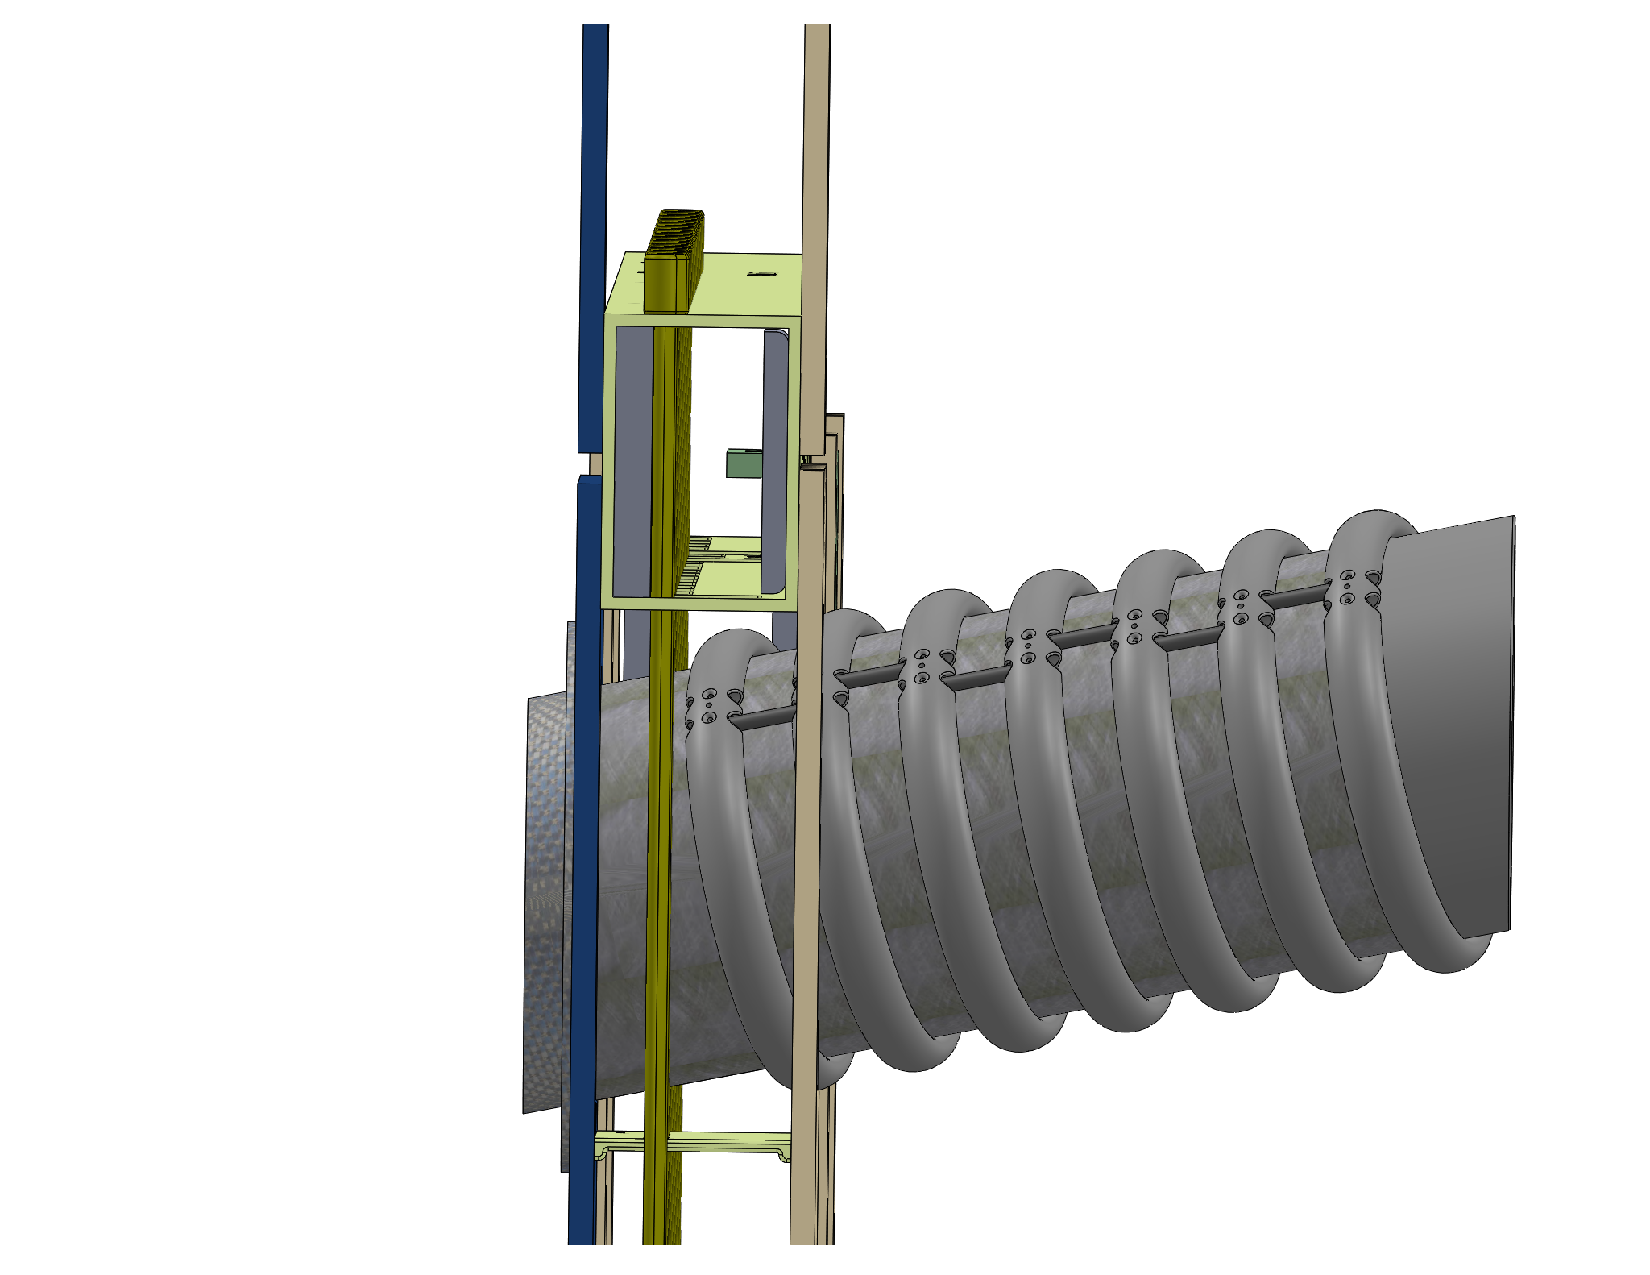
\includegraphics[width=0.5\linewidth]{beamplug-fc2.pdf}
%\end{cdrfigure}
